% background
% brief review of previous research (cite)
% reson why the research was undertaken
% Hypothesis
% explenation of techniques and why they ve been chosen
% objectives = what you hope to achieve
% brief reference to the main outcome

%$\ce{CdS_x Se_{1-x}/ZnS}$

% \begin{figure*}
%   \centering
%   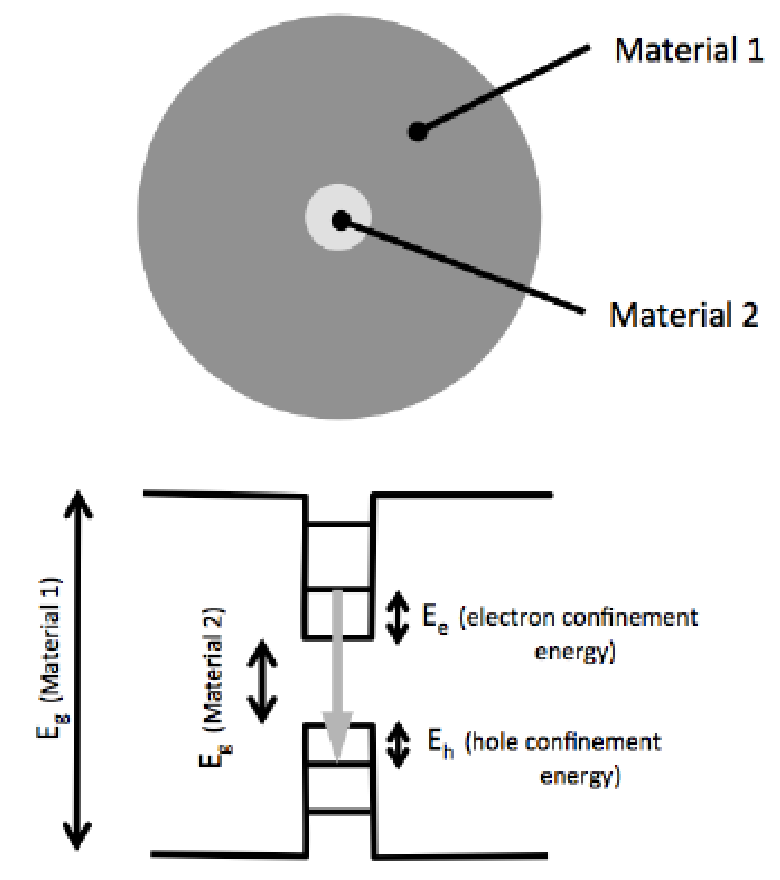
\includegraphics[width=0.35\textwidth]{graphics/QD.png}
%   \caption[width=0.4\textwidth]{\cite{instruction}.}
%   \label{fig:QD}
% \end{figure*}

\section{Introduction}
\label{sec:Introduction}
% Application of low-dimensional organic semiconductors in spintronics
As part of the course "Semiconductors and nanostructures" the aim of this short report is to get a deeper inview into a specific subject of the course, such as getting an understanding of the current state of the art research.
Therefore, I want to focus on the application of low-dimensional organic semiconductors in spintronics, their benefits compared to conventional semiconductors and their preperation up to a functioning circuit.
The idea of spintronics will be introduced shortly and only in the parts which are used in the example funtionality of a spin-OLED, as spintronics itself is an upcoming reseach field with several different paradigms and branches.

\section{Spintronics}
\label{sec:spintronics}

The word "spintronics" sets together from the words "spin" and "electronics", and thus means the exploitation of electrons spin instead of its charge for computing.
The most famous example of metal based spintronics in use is the giant magnetorestance effect (GMR), which is used in hard disk drives.
Here, the resitance of a multilayer device depends strongly on the relative magnetization of two magnetic layers stacked on each other \cite{perovskite}.
In spintronics information can be stored in a spin state of an electron, which is described by magnetism.
The information can travel by spin-polarized charge or by spin-waves, which are collective oscillations of electrons doing precession motion around a fixed direction of magnetization \cite{clocks}.
Here, the properties of either wave amplitude or phase, or a combination of both can code the information states, as depicted in figure \ref{fig:spin-coding}.

\begin{figure}
    \centering
  \captionsetup{width=0.7\linewidth}
  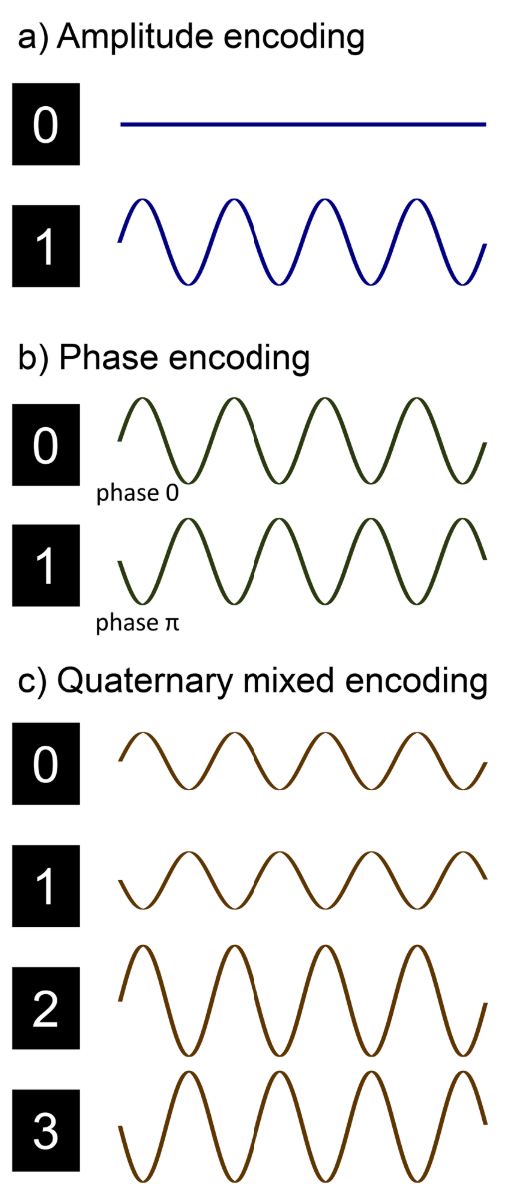
\includegraphics[width=0.4\textwidth]{graphics/spin-code.png}
  {Comparison of shemes to encode information in spin-waves \cite{computing}.}
  \label{fig:spin-coding}
\end{figure}

In order to process information other pyhsical interactions have to be considered, such as interference, spin-orbit-coupling and quantum magnetic interactions \cite{perovskite}.
One can see, that easily more than a binary coding system can be introduced. 
Further it is imaginable to use the same device simultaniously for several calculations, as the properties of a wave allow superposition \cite{computing}.

Using spin-waves for information transport gives the oportuntity of low-energy-consumption, non-volatile and less material consuming computing \cite{clocks}. 
In order to built a interconnect a full set of boolean logic circuit to a functioning, complex device, the biggest problem is the small ($\sim\SI{10}{\micro\meter}$ \cite{computing}) propagation, and exponentially decreasing attenuation length of spin waves in metals, which classically may be solved by rather complicated amplification steps (compare \cite{clocks}).
The megnetic damping of the spin wave as well as the group velocity are dependant on the material and geometry of the waveguide \cite{computing} \cite{SC-spintronics}.
Another problem is the interconnection between classical, charge-based circuits and spintronic devices, which bases on magnetic-coupling \cite{clocks}. 
Here, there are different strategies for so called spin-injection \cite{perovskite}, which will be more elaborated in the next chapter about organic spintronics.
To optimate these processes, a good understanding of spin-relaxation and spin-transport mechanisms in metals and semiconductors is the basis, so reseachers invested a lot of time in these fields recently \cite{perovskite}.
Further, the impact of dimensionality, defects and the band structure are in big interest \cite{perovskite} \cite{SC-spintronics}.



\section{Organic spintronics}
\label{sec:org-spintronics}
% criteria for material choice and example materials
On the search for spin-waveguides, thus for materials throug which a spinwave can propagate long distances without loosing coherence or intensity, organic semiconductors became promising candidates.
In more detail, $\pi$-conjugated organic semiconductors are composed of elements with low atomic number $Z$.
Thus, the spin-orbit coupling proportional to $Z^4$ \cite{valve}, which mainly is in charge of the spin-wave damping, is small \cite{appl-organic}.

%theory of charge transport in OSC
About the spin-dependent charge transport in OSC we know, that it is much more complicated than the band-like transport in non-organic semiconductors.
The delocalized carriers inside the molecules are coupled with weak van-der-Vaals interconections between the molecules, what heavily limits the overall carrier mobility.
The carriers propagate by random thermally assisted hopping between pseudo-localized states.
In addition, the typical band-like conduction of LUMO and HOMO are taking place inside the molecule and can be spin-polarized.
Defect and interface states may have to be taken into account depending on the materials quality \cite{valve} \cite{perovskite}.

The spin trannsport can be rationalized by the Einsteins`s relationship $\lambda_e = \sqrt{(D_\text{hop} + D_\text{ex})\tau_s}$,
where $\lambda_s$ is the spin diffusion, $D_\text{hop}$ the diffusion coefficient for hopping mode spin transport (phonon-assisted tunneling), $D_\text{ex}$ the diffusion coefficient for spin transport following exchange coupling mode and $\tau_s$ is the spin relaxation time \cite{perovskite}.
The excange coupling, which occurs for high carrier concentration provides faster spin diffusion, as it is decoupled from charge transport.


In order to measure the spin transport, a spin valve setup can be used, where the spin-transport layer is sandwiched between to ferromagnetic electrodes, as seen in figure \ref{fig:valve}.
Here, spin-polarised electrons are injected into the OSO thin film and detected from the second electrode \cite{appl-organic}.
By inverting the direction of the external magnetic field, the two electrondes get magnetized aprallel (P) or antiparallel (AP).
So, quantitively the GMR mentioned in chapter \ref{sec:spintronics} can be expressed by the magnetoresistance $MR = (R_\text{AP}-R_\text{P}/R_\text{AP})$.
The thickness of the tested OSC layer can be considered as the spin transport length \cite{appl-organic}.

In more detail, a reliable spin valve preparation where penetration of metal atoms into the OSC has to be impeded.
This turns out to be a big technical difficulty for thin film fabrication as OSCs are soft materials. 

\begin{figure}
    \centering
  \captionsetup{width=0.7\linewidth}
  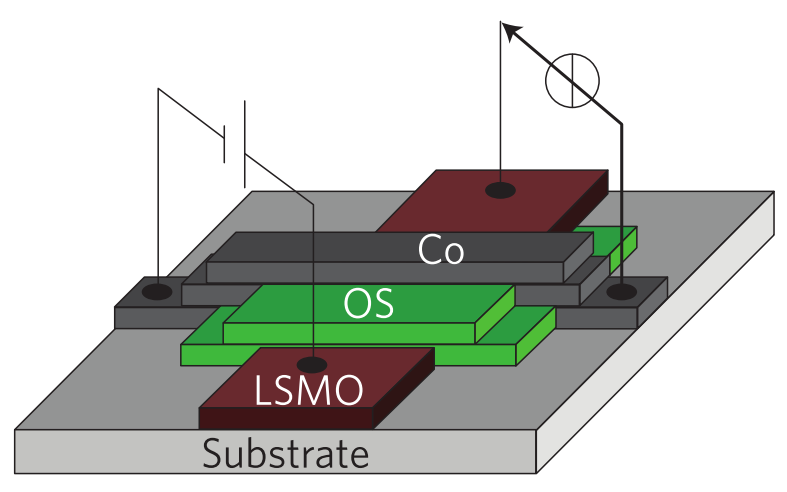
\includegraphics[width=0.4\textwidth]{graphics/valve.png}
  {Spin valve where a OSC (green) is stacked between two ferromagnetic kathodes (LSMO and Copper) \cite{valve}.}
  \label{fig:valve}
\end{figure}

Nethertheless, using the spin valve it becomes possible to anayze the impact of molecular sturcture, composition and aggregation structure, which all have vast impact on the spin-transport quality \cite{appl-organic}.

% Examples of different material candidates


In addition, organic semiconductors (OSCs) have a set of unique properties such as flexibility, tailorability and photo-electric properties \cite{appl-organic}.
These photo-electric function for example can be used to integrate detector or sensor functions directly into a spintronic circuit.

Another special class of application are electrodes, wher organic-based magnets can be useful to reduce the contact resitance.



\section{low-dimensional and monocrystalin org. semiconductors}
\label{sec:2D}

\section{Spin-OLED}
\label{sec:device}
A lot of organic based spintronics devices do still exist only in concept.
They can be devided into two classes which are magnetic resonant tunnel stuctures or bipolar magnetic diodes and transistors \cite{SC-spintronics}
% Architecture and manufacturing
% other possible devices

\section{Alternative materials}
\label{sec:alternative}
% Perovskites


